\chapter{Features of the research framework}

% INTRODUCTION %

In this chapter we describe the \<framework> that we have developed to perform user-based online validation for researches in procedural content generation of multiplayer levels for Firsts Person Shooters. In the first partition we give an overview of the framework, of its features and of its components, analyzing them one by one in the following sections.

% FRAMEWORK OVERVIEW 

\section{Overview}

We designed our framework with the objective of providing a valid alternative to the games currently employed as a validation tool in this research field. All the available options, like \<Cube 2: Sauerbraten>: are powerful tools to perform validation via artificial agents, but they are not suitable for user-based validation. A data-collection campaign based on these games requires to download the game or to take part in real-life play-test sessions, but these options discourage potential participants because they are significantly time-consuming. For this reason, we decided to develop a framework that is as light as possible, with a WebGL build weighting less than 10MB that can be played using any browser. The framework was developed with Unity.

\par

Since the purpose of this tool is to be used in research, we decided to support many map representation formats used in previous works and we designed our framework to be as modular, expansible and configurable as possible.

\section{The framework structure}

The framework collects data by assigning to the users \<matches> to play. A match is defined by the \<game mode> and by the \<map type>: which in turn is defined by the \<map topology> and by the \<map appearance>. The \<map topology> defines how the map is going to \<be> and depends on the algorithm used to generate it, whereas the \<map appearance> defines how the map is going to \<look> and depends on how the map is assembled. This implies that the map type defines a whole array of procedurally generated maps that share the same topology and appearance. Therefore, when referring to a match we are considering a specific game-mode played in a procedurally generated map. If needed, it is possible to use a pre-generated map instead of generating a new one, by providing it as input in one of the supported formats. In this case the \<map topology> defines how to interpret the input, that is then displayed considering the \<map appearance>.

\par

A match is defined by combining different modular \<Manager> objects, each of which controls a different aspect of the match. To assure their interchangeability, most modules are defined by their own abstract class.

\subsection{The Game Manager}

The \<Game Manager> is the module responsible for the overall behavior of a match. Each game mode consists in a different implementation of the \<Game Manager>. It leans on the \<Map Manager> for the generation and the assembly of the map and on the \<Spawn Point Manager> for the spawn of entities. The \<Game Manager> controls the life-cycle of the match, that can be divided in the following phases:

\begin{itemize}
\item \<Setup>: all the modules are initialized.
\item \<Generation>: the \<Map Manager> generates or imports the map and assembles it.
\item \<Ready>: the \<Game Manager> displays a countdown announcing the start of the game.
\item \<Play>: the \<Game Manager> handles the game while the \<Experiment Manager> logs the actions of the player, if needed. This phase continues until an end condition is satisfied.
\item \<Score>: the \<Game Manager> stops the game and displays the final score.
\end{itemize}

\subsection{The Spawn Point Manager}

The \<Spawn Point Manager> contains a list of all the spawn points displaced on the map, that is populated during the \<Generation> phase by the \<Game Manager>. When the \<Game Manager> needs to spawn an entity, the \<Spawn Point Manager> provides a random spawn point from the ones that have not been used in a certain amount of time. If no spawn point meets this condition, the extraction is made from the complete pool.

\subsection{The Map Manager}

The \<Map Manager> controls the generation, the import and the assembly of the map and the displacement of objects inside it. It leans on the \<Map Generator> for the generation, on the \<Map Assembler> for the <assembly>\footnote{With \<assembly> we mean the operation of creating a 3D model of the map starting from its matrix representation.}, on the \<Object Displacer> for the \<displacement>\footnote{With \<displacement> we mean the operation of placing the 3D models of the objects in the assembled map, according to their position defined by the \<Map Generator> trough a \<positioning> algorithm.}, whereas it performs the import itself. If the map is provided as input, the \<Map Generator> is not called.

\par

Maps are structured as a grid of orthogonal \<tiles> and are represented as matrices of characters, where each cell corresponds to a specific \<tile>. Depending on the character, a cell can represent a wall, a floor or an object on the floor. If a cell corresponds to a wall we say it is \<filled>: if it corresponds to a floor we say it is \<empty>.

\subsection{The Map Generator}

The \<Map Generator> controls the generation of the map. Each implementation of the \<Map Generator> defines a different topology depending on the used generation algorithm and on how its parametric setting are tuned. Some of these setting are shared by all the implementations, whereas some of them are implementation-specific.

\par

The shared settings are used to define the size of the map and its encoding, to define the objects and to impose some constraints on their positioning:

\begin{itemize}
\item \<Width>: the width of the matrix that represents the map.
\item \<Height>: the height of the matrix that represents the map.
\item \<ObjectToObjectDistance>: the minimum number of cells that must separate two objects. 
\item \<ObjectToWallDistance>: the minimum number of cells  that must separate an objects and a wall.
\item \<BorderSize>: the width of the border placed all around the map once it has been generated, expressed in number of cells.
\item \<RoomChar>: the character used to represent a clear cell where the player can walk.
\item \<WallChar>:  the character used to represent a filled cell where the player can not walk.
\item \<MapObjects>: a list of the objects that must be placed in the map.
\end{itemize}

The objects contained in \<MapObjects> can represent spawn points, resources or decoration. They have the following properties:

\begin{itemize}
\item \<ObjectChar>: the character used to represent the object.
\item \<NumObjPerMap>:  the number of objects of that kind that must be placed in the map.
\item \<PlaceAnywhere>: if this value is set to true, the restriction on the distance from the walls is ignored.
\item \<PositioningMode>: the algorithm used to position the object in the map.
\end{itemize}

The framework provides three different algorithms to position the objects inside the map:

\begin{itemize}
\item \<Rain>: positions the objects selecting random cells from the ones that are empty and satisfy the  \<ObjectToWallDistance> constraint.
\item \<Rain Shared>: positions the objects selecting random cells from the ones that are empty and satisfy the  \<ObjectToWallDistance> constraint and the \<ObjectToObjectDistance> constraint on the objects that have been placed using \<Rain Shared>.
\item \<Rain Distanced>: positions the objects selecting random cells from the ones that are empty and satisfy the  \<ObjectToWallDistance> constraint and the \<ObjectToObjectDistance> constraint on the objects with the same \<ObjectChar>.
\end{itemize}

All of the following implementations of the \<Map Generator> are deterministic, since they require a \<seed> value as input that constrains the output to a specific map.

% CELLULAR GENERATOR %

\subsubsection{Cellular Generator}

The \<Cellular Generator> employs a parametric \<cellular automaton>\footnote{A \<cellular automaton> consists of a grid of cells, each in one of a finite number of states, such as on and off. For each cell, a set of cells called its neighborhood is defined, usually composed by the ones that share at least one vertex with it (referred as \<8-neighbors>). Given the current state of the grid, a new generation is created, according to some fixed rule that determines the new state of each cell depending on the current state of the cell and of its neighbors.} to generate a natural looking map. 

\par

The algorithm starts by filling some tiles of the map selected at random, then it applies the cellular automaton for a certain number of generations and finally it performs some refinements (for more details, see algorithm \ref{alg:cellular}). The resulting topology depends on the following parameters:

\begin{itemize}
\item \<RandomFillPercent>: the percentage of tiles that are randomly filled during the initialization of the algorithm. High values promote narrow spaces, small values promote wide open areas.
\item \<SmoothingInteration>: the number of generations the cellular automaton is ran for. High values penalize small features and make the walls smoother. 
\item \<NeighbourTileLimitLow>: the minimum number of neighbors a cell must have to became filled. Its value must be lesser or equal than the one of \<NeighbourTileLimitHigh>. The map becomes noisier the more they diverge.
\item \<NeighbourTileLimitHigh>: the maximum number of neighbors a cell must have to became empty.
\item \<WallThresholdSize>: the minimum number of cells that an isolated filled region must include to not be deleted. High  values penalize small filled regions.
\item \<RoomThresholdSize>: the minimum number of cells that an isolated void region must include to not be deleted. High  values penalize small empty regions.
\item \<PassageWidth>: the width of a passage connecting two different areas, expressed in number of cells.
\end{itemize}

Figure \ref{fig:cellulars} shows how these parameters influence the topology of a map.

\begin{algorithm}[tp]
\SetAlgoLined
\caption{Cellular generation algorithm.}
\algorithmfootnote{This algorithm is a modified version of the one proposed by Sebastian Lague\cite{lague}.}
\label{alg:cellular}

\For{every cell in the map}{
	empty the current cell\;
}

\While{percentage of filled cells $<$ RandomFillPercent} {
	select a random cell\;
	fill the selected cell\;
}

\For{generation from 0 to SmoothingIterations} {
	\For{every cell in the map}{
		count the 8-neighbors of the cell\;
		\If{cell neighborhood $>$ NeighbourTileLimitLow}{
  			mark the current cell as filled for the next generation\;
   		}
		\If{cell neighborhood $<$ NeighbourTileLimitHigh }{
  			mark the current cell as empty for the next generation\;
   		} 
	}
	update the map to the next generation\;
}

\For{every connected region of empty cells}{
	\If{\#cells in the region $<$ RoomThresholdSize}{
		fill all the cells in the region\;
	}
}

\For{every connected region of filled cells}{
	\If{\#cells in the region $<$ WallThresholdSize}{
		empty all the cells  in the region\;
	}
}

connect all the regions composed by empty cells\;
place the objects\;

\end{algorithm}

\begin{figure}[tp]
	\centering
  	\begin{subfigure}[t]{0.325\linewidth}
		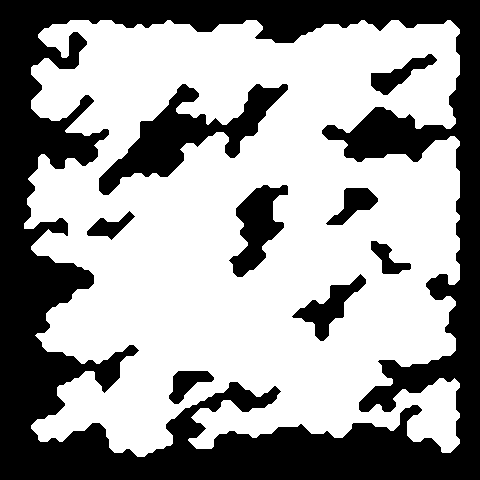
\includegraphics[width=\linewidth]{cellular_default}
     		\caption{Cellular map generated with the default settings.}
 	\end{subfigure}
  	\begin{subfigure}[t]{0.325\linewidth}
    		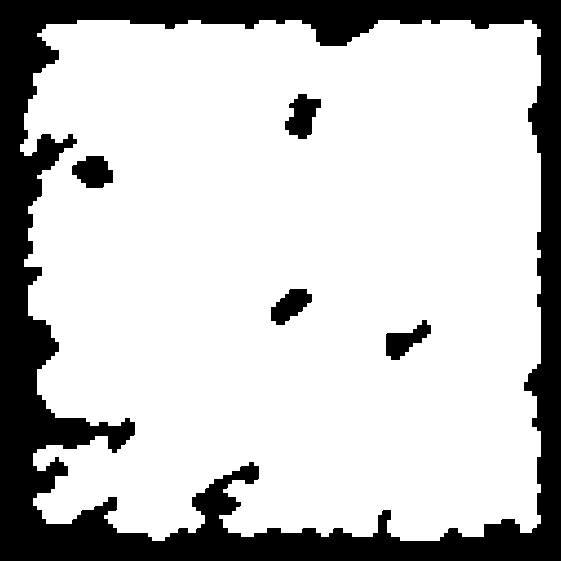
\includegraphics[width=\linewidth]{cellular_rfp40}
    		\caption{Cellular map generated with $Ran\-dom\-Fill\-Per\-cent = 40\%$.}
  	\end{subfigure}
  	\begin{subfigure}[t]{0.325\linewidth}
    		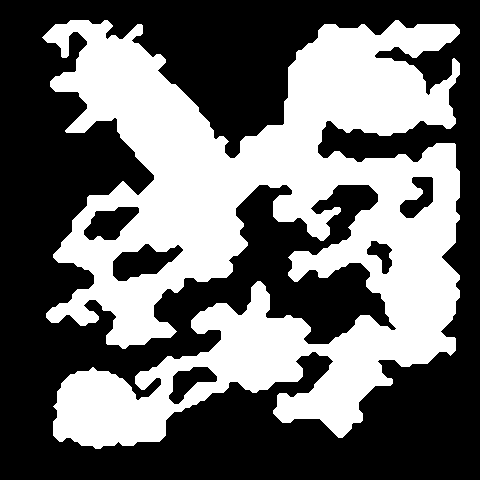
\includegraphics[width=\linewidth]{cellular_rfp50}
    		\caption{Cellular map generated with $Ran\-dom\-Fill\-Per\-cent = 50\%$.}
  	\end{subfigure}
  	\begin{subfigure}[t]{0.325\linewidth}
		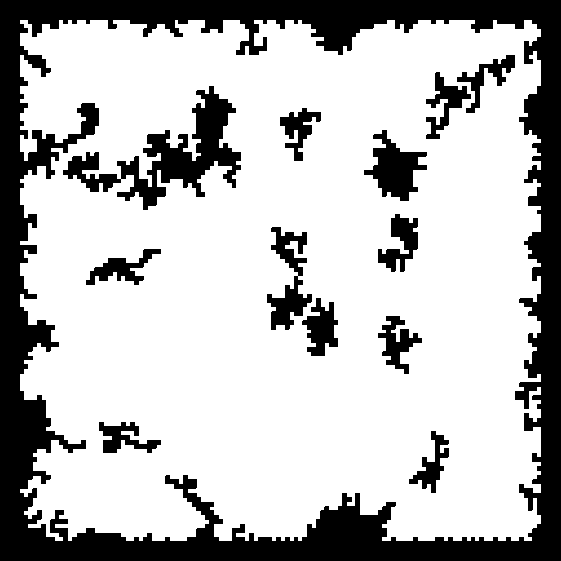
\includegraphics[width=\linewidth]{cellular_si0}
     		\caption{Cellular map generated with $Smooth\-ing\-It\-er\-a\-tions = 0$.}
 	\end{subfigure}
  	\begin{subfigure}[t]{0.325\linewidth}
    		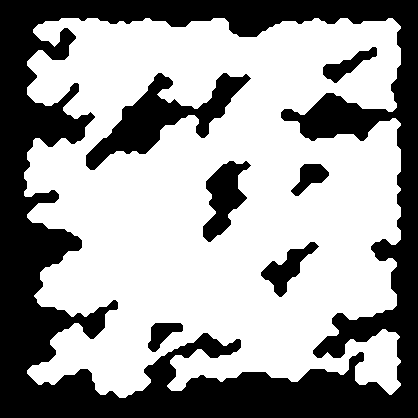
\includegraphics[width=\linewidth]{cellular_si3}
     		\caption{Cellular map generated with $Smooth\-ing\-It\-er\-a\-tions = 3$.}
  	\end{subfigure}
  	\begin{subfigure}[t]{0.325\linewidth}
    		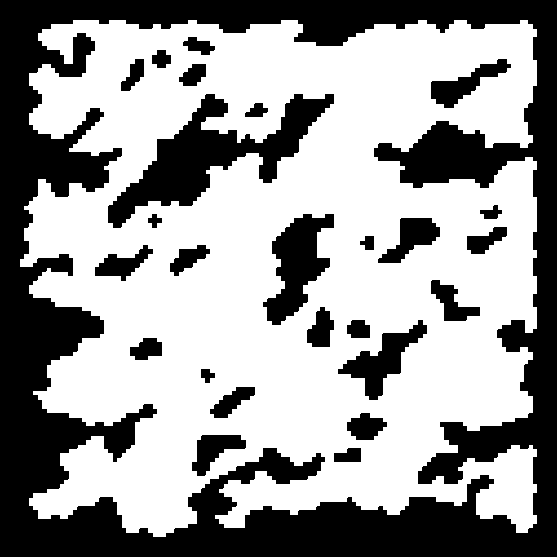
\includegraphics[width=\linewidth]{cellular_wts5}
     		\caption{Cellular map generated with $Wall\-Thresh\-old\-Size = 5$.}
  	\end{subfigure}	
	\caption{Some maps generated by the Cellular Generator using ''\<ANotSoRandomSeed>'' as seed, but different settings.}
	\caption*{By default, the Cellular Generator has \<RandomFillPercent> set to $45\%$, \<SmoothingIterations> set to $2$,  \<NeighbourTileLimitHigh> set to $4$,  \<NeighbourTileLimitLow> set to $4$,  \<WallThresholdSize> set to $40$ and \<RoomThresholdSize> set to $100$.}
	\label{fig:cellulars}
\end{figure}

% DIVISIVE GENERATOR %

\subsubsection{Divisive Generator}

The \<Divisive Generator> employs a \<binary space partitioning algorithm> to generate a man-made looking map.

\par

The algorithm starts by obtaining partitions of the map by recursively dividing it in two sides of random size along one of the axes, then it selects some of these partitions as rooms and finally it connects them with corridors (for more details, see algorithm \ref{alg:divisive}). The resulting topology depends on the following parameters:

\begin{itemize}
\item \<RoomDivideProbability>: probability of a partition being divided again. High values promote small rooms.
\item \<MapRoomPercentage>: minimum percentage of tiles of the map that must be empty. High values promote close rooms separated by walls, low values promote distant rooms connected by corridors.
\item \<DivideLowerBound>: minimum division point expressed as percentage of the dimension of the room.
\item \<DivideUpperBound>: maximum division point expressed as percentage of the dimension of the room.
\item \<MinimumRoomDimension>: minimum width expressed in number of cells that a partition must have to be divided again. High values promote large rooms.
\item \<MinimumDepth>: the minimum number of recursive divisions that each partition must have experienced.
\item \<PassageWidth>: the width expressed in number of cells of the corridors connecting the rooms.
\item \<MaxRandomPassages>: the number of additional corridors to place, if possible, once that all the rooms are connected.
\end{itemize}

Figure \ref{fig:divisives} shows how these parameters influence the topology of a map.

\begin{algorithm}[tp]
\SetAlgoLined
\caption{Divisive generation algorithm.}
\label{alg:divisive}

\For{every cell in the map}{
	fill the current cell\;
}

initialize the partitions list\;
DivideRoom(map, 0)\;

\While{percentage of empty tiles $<$ MapRoomPercentage}{
	extract a partition from the partitions list\;
	make the partition a room\;
	empty the tiles in the room\;
}

connect the rooms; 

\While{all the rooms are not directly connected \And \#placed additional corridors $<$ MaxRandomPassages}{
	add an additional corridor between two rooms;
}

place the objects\;

\hrulefill

\SetKwProg{Fn}{Function}{ is}{end}
\Fn{DivideRoom(section, depth)}{
	\eIf{(true with probability roomDivideProbability \And partition width $>$  minimumDividableRoomDimension \And partition heigth $>$ minimumDividableRoomDimension) \Or depth $<$  minimumDepth} {
		\eIf{previous division was horizontal} {
 			perform a random vertical division between \<divideLowerBound> and \<divideUpperBound>\;
		} {
 			perform a random horizontal division between \<divideLowerBound> and \<divideUpperBound>\;
		}
		DivdeRoom(first sub-section, depth + 1)\;
		DivdeRoom(second sub-section, depth + 1)\;
	}{
		add the partition to the partitions list;
	}	
}

\end{algorithm}

\begin{figure}[tp]
	\centering
  	\begin{subfigure}[t]{0.325\linewidth}
		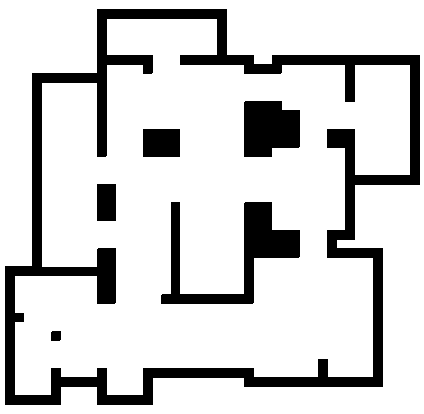
\includegraphics[width=\linewidth]{divisive_default}
     		\caption{Divisive map generated with the default settings.}
 	\end{subfigure}
  	\begin{subfigure}[t]{0.325\linewidth}
    		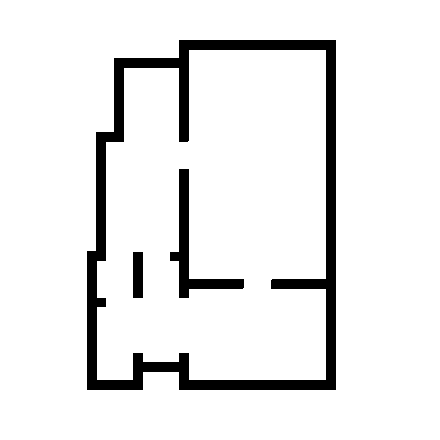
\includegraphics[width=\linewidth]{divisive_rdp20}
    		\caption{Divisive map generated with $Room\-Di\-vide\-Prob\-a\-bil\-i\-ty = 20\%$.}
  	\end{subfigure}
  	\begin{subfigure}[t]{0.325\linewidth}
    		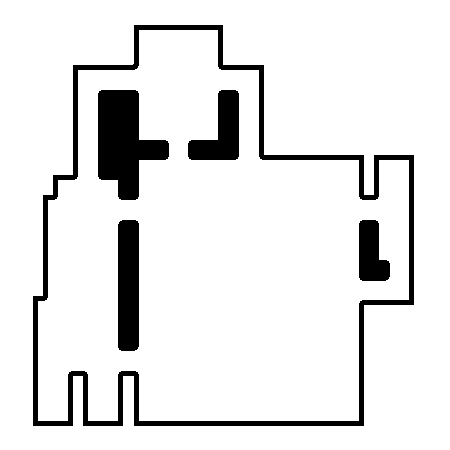
\includegraphics[width=\linewidth]{divisive_md1}
    		\caption{Divisive map generated with $Min\-i\-mum\-Depth = 1$.}
  	\end{subfigure}
  	\begin{subfigure}[t]{0.325\linewidth}
		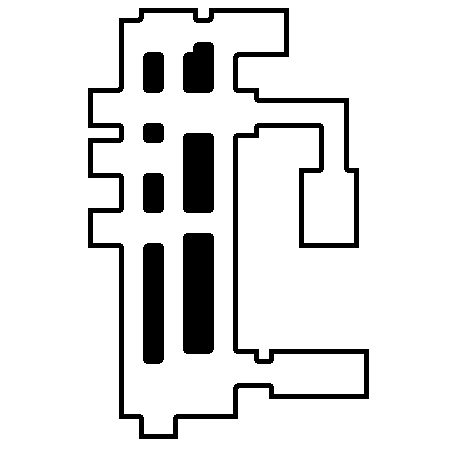
\includegraphics[width=\linewidth]{divisive_md8}
     		\caption{Divisive map generated with $Min\-i\-mum\-Depth= 8$.}
 	\end{subfigure}
  	\begin{subfigure}[t]{0.325\linewidth}
    		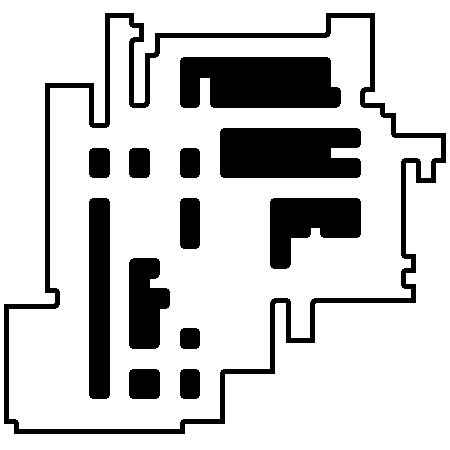
\includegraphics[width=\linewidth]{divisive_mrd1}
     		\caption{Divisive map generated with $Min\-i\-mum\-Room\-Di\-men\-sion = 1$.}
  	\end{subfigure}
  	\begin{subfigure}[t]{0.325\linewidth}
    		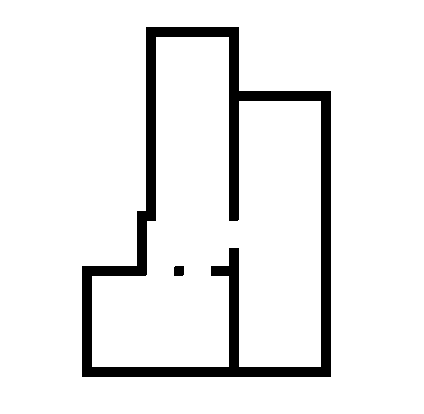
\includegraphics[width=\linewidth]{divisive_mrd7}
     		\caption{Divisive map generated with $Min\-i\-mum\-Room\-Di\-men\-sion = 7$.}
  	\end{subfigure}	
	\caption{Some maps generated by the Divisive Generator using ''\<AModeratelyRandomSeed>'' as seed, but different settings.}
	\caption*{By default, the Cellular Generator has \<Room\-Di\-vide\-Prob\-a\-bil\-i\-ty> set to $80\%$, \<Map\-Room\-Per\-cent\-age> set to $90\%$,  \<Di\-vide\-Low\-er\-Bound> set to $10\%$,  \<Di\-vide\-Up\-per\-Bound> set to $90\%$,  \<Min\-i\-mum\-Room\-Di\-men\-sion> set to $3$, \<Min\-i\-mum\-Depth> set to $4$, \<Pas\-sage\-Width> set to $3$ and \<Max\-Ran\-dom\-Pas\-sages> set to $12$.}
	\label{fig:divisives}
\end{figure}

% DIGGER GENERATOR &

\subsubsection{Digger Generator}

The \<Digger Generator> employs a simple algorithm to generate a man-made looking map.

\par

The algorithm is iterative and its state is defined by the current cell and by the current direction, that together with a randomly selected action determine the next cell that the algorithm is going to visit. Starting from the central cell of a completely filled map, at each iteration the algorithm empties the current cell and randomly decides if moving forward, turning left and then moving forwards, turning right and then moving forward, jumping to a random visited cell or placing a flight of stairs, if controlled by a \<Multi-Level Generator>. The algorithm stops when a certain percentage of cells has been emptied. The resulting topology depends on the following parameters:

\begin{itemize}
\item \<ForwardProbability>: probability of moving forward in the next iteration. High values promote long corridors. 
\item \<LeftProbability>: probability of moving forward in the next iteration. High values promote wide open areas. 
\item \<RightProbability>: probability of moving rigthward in the next iteration. High values promote wide open areas. 
\item \<VisitedProbability>: probability of jumping to a visited cell in the next iteration. High values promote a more complex topology. 
\item \<StairProbability>:  probability of placing a flight of stairs.
\item \<RoomPercentage>: percentage of tiles of the map that must be empty.
\end{itemize}

\begin{figure}[tp]
	\centering
  	\begin{subfigure}[t]{0.48\linewidth}
		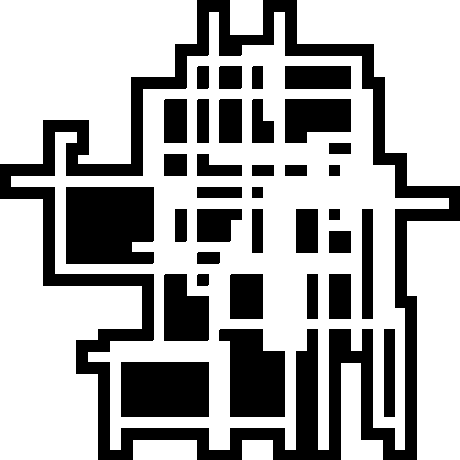
\includegraphics[width=\linewidth]{digger_default}
     		\caption{Digger map generated with the default settings.}
 	\end{subfigure}
  	\begin{subfigure}[t]{0.48\linewidth}
    		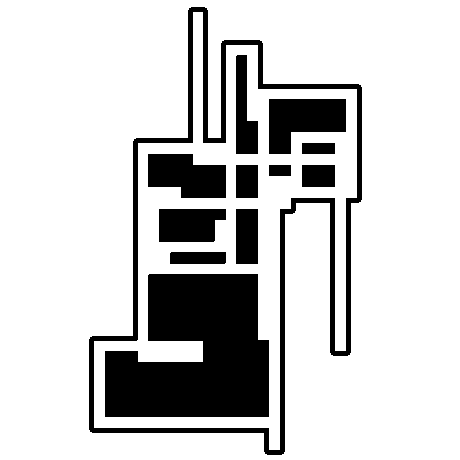
\includegraphics[width=\linewidth]{digger_roomp20}
    		\caption{Digger map generated with $Room\-Per\-cent\-age = 20\%$.}
  	\end{subfigure}
  	\begin{subfigure}[t]{0.48\linewidth}
    		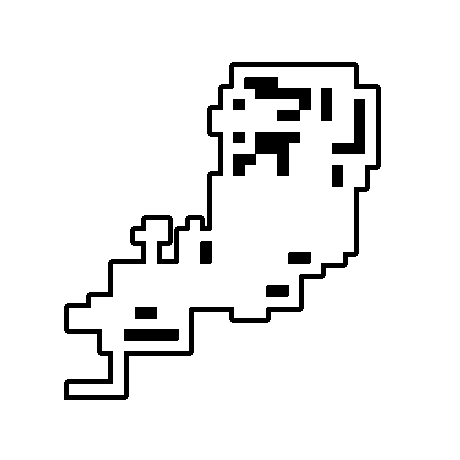
\includegraphics[width=\linewidth]{digger_fp60}
    		\caption{Digger map generated with $For\-ward\-Prob\-a\-bil\-i\-ty = 60\%$, $Right\-Prob\-a\-bil\-i\-ty = 19\%$ and $Left\-ward\-Prob\-a\-bil\-i\-ty = 19\%$.}
  	\end{subfigure}
  	\begin{subfigure}[t]{0.48\linewidth}
		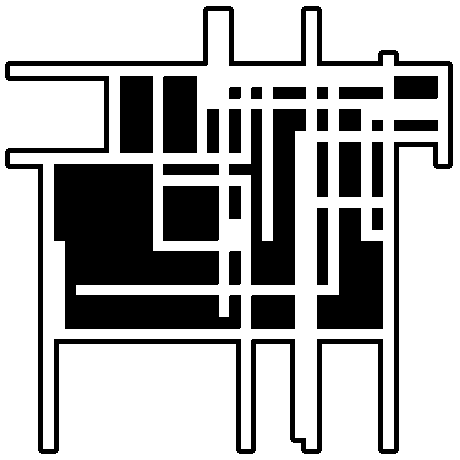
\includegraphics[width=\linewidth]{digger_fp96}
    		\caption{Digger map generated with $For\-ward\-Prob\-a\-bil\-i\-ty = 96\%$, $Right\-Prob\-a\-bil\-i\-ty = 1\%$ and $Left\-ward\-Prob\-a\-bil\-i\-ty = 1\%$.}
 	\end{subfigure}
	\caption{Some maps generated by the Digger Generator using ''\<AFairlyRandomSeed>'' as seed, but different settings.}
	\caption*{By default, the Digger Generator has \<For\-ward\-Prob\-a\-bil\-i\-ty> set to $90\%$, \<Left\-Prob\-a\-bil\-i\-ty> set to $4\%$, \<Right\-Prob\-a\-bil\-i\-ty> set to $4\%$, \<Vis\-it\-ed\-Prob\-a\-bil\-i\-ty> set to $2\%$, \<Stair\-Prob\-a\-bil\-i\-ty> set to $0\%$ and \<Room\-Per\-cent\-age> set to $50\%$.}
	\label{fig:diggers}
\end{figure}


Figure \ref{fig:diggers} shows how these parameters influence the topology of a map.

% MULTI-LEVEL GENERATOR %

\subsubsection{Multi-level Generator}

\subsection{The Map Assembler}

The \<Map Assembler> controls the assembly of the map. Each different implementation of the Map Assembler corresponds to a different appearance.

\par

They are light and simple.

% MESH ASSEMBLER %

\subsubsection{Mesh Assembler}

% PREFAB ASSEMBLER %

\subsubsection{Prefab Assembler}

\subsection{The Object Displacer}

The \<Object Displacer> associates a character that represents neither a wall or a clear cell to the corresponding object, displacing it in the correct position. During this process, it populates a dictionary containing all the objects in the map divided by category, that is used by the \<Game Manager> to populate the list of spawn points used by the \<Spawn Point Manager>.

% MAP REPRESENTATION %

\section{Map representation}

% WEAPONS AND OBJECTS %

\section{Weapons and objects}

% GAME MODES %

\section{Game modes}

% LOGGING %

\section{Logging}

% EXPERIMENT MANAGEMENT %

\section{Experiment management}
